\chapter{Algorithmes et Analyse}




\section{Descripteurs}
Pour pouvoir appliquer notre mesure de similarité entre deux images et calculer les poids de nos particules, on a besoin de pouvoir extraire de l'information de nos images. Ainsi nous allons utiliser des descripteurs. \\
Un descripteur est un morceau d'information extrait d'une image sous forme de vecteur. Il permettra de reconnaitre un motif ou une structure spécifique au cours de notre vidéo. Pour calculer un descripteur on s'appuie sur l'information bas niveau de nos images (valeur des pixels, contours, gradients, ...).

\subsection{Histogramme de gradient orienté}

Nous utiliserons en particulier les histogrammes de gradients orientés (HOG) qui sont des descripteurs proposés par Navneet DALAL et Bill TRIGGS \cite{dalal_histograms_2005}. Ils correspondent à la distribution de l'orientation des contours locaux d'une image. \\

Les HOG sont calculés par DALAL et TRIGGS ainsi : \\

Une première étape de pré-traitement de l'image afin de normaliser les couleurs et d'appliquer une correction gamma à celle-ci puis la convertir en niveau de gris. Ici la normalisation du HOG est suffisante et cette étape est donc facultative, on s'est contenté de la conversion en niveau de gris. \\

L'étape suivante est le calcul de la carte des gradients en x et en y qui correspondent respectivement à la variation horizontal et vertical des gradients. On effectue une convolution centrée sur le pixel cible. Parmi les différents filtres possibles, les masques que nous utilisons sont $[-1, 0, 1]$ pour les gradients en x et $[-1, 0, 1]^{T}$ pour les gradients en y, aussi appelés filtres de Sobel. Ces masques se sont révélés plus performants dans la littérature \cite{dalal_histograms_2005}.\\

À partir de ces deux cartes de gradients on pourrait calculer la carte des modules des gradients. Néanmoins, afin d'augmenter l'efficacité du descripteur, le HOG n'est pas directement calculer à partir de l'image.\\

En effet l'image est diviser en "cellules", elle-même regroupées en "blocs". On choisit des cellules de 6*6 pixels et des bloc de 3*3 cellules.\\

Pour chaque blocs, on calcule le HOG de chaque cellule. Le HOG du bloc correspond à la concaténation du HOG des cellules le composant. Pour une meilleure invariance face à l'illumination et à l'ombrage on effectue une normalisation du HOG du bloc (norme euclidiennne). Pour un vecteur x, on a :

\[ \sum_{k=0}^{n} (x_{k})^{2} \]

Donc le HOG de l'image est la concaténation de l'ensemble des HOG de chacun de ses blocs.

\begin{figure}[!htbp]
\center
	\subfloat{{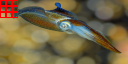
\includegraphics[height=3cm]{Squid_colors_2resized.png}}}
\caption{Bloc d'un HOG.}
\label{fig:cuttlefish_bloccells}
\end{figure}

Les histogrammes sont construits grâce au mesures des angles des gradients et à leurs intensités. De la même manière qu'avec la taille des blocs et des cellules, on doit choisir la structure de notre histogramme. Étant donnés que nous travaillons sur des angles, nous choisirons un histogramme à neuf classes et nous utiliserons des angles non signés (compris entre $[0; 180°]$).
Ainsi pour un pixel $p(x,y)$ l'angle est définis par :

\[ angle_{p} = |\arctan (\grad y, \grad x)*\frac{180}{\pi}| \]

De même que son intensité par :

\[ intensite_{p} = \sqrt{\grad x^{2} + \grad y^{2}} \]

Pour chaque pixel, on répartit son intensité proportionnellement dans les deux classes les plus proche de l'angle qui lui est associé. 
Par exemple, prenons $\grad x = 10$ et $\grad y = 10$ on obtient un intensité d'environ $14.14$ et un angle de $45°$. De cette manière la classe centrée en $40$ recevra les trois quarts ($1 - |\frac{5}{20}|$)et la classe centrée en $60$ recevra le quart restant($1 - |\frac{15}{20}|$) de l'intensité.\\

% Note : prendre gradx = grady = sqrt(2) est plus stylé mais je sais pas si c'est sage

Enfin pour affiner notre descripteur nous effectuerons le déplacement du bloc suivant :

\[ \frac{T_{cellule} * T_{bloc}}{2} \]

$T_{cellule}$ est la taille en pixel de la cellule,
$T_{bloc}$ est la taille en nombre de cellule d'un côté du bloc.
Ainsi on a : $\frac{6*3}{2} = 9$, de plus, un bloc faisant plus de 9 pixels de côté, on a un chevauchement des blocs et donc des pixels pris en compte plusieurs fois. Cela permet au vecteur de mieux caractériser l'image cible.

\begin{figure}[!htbp]
\center
	\subfloat{{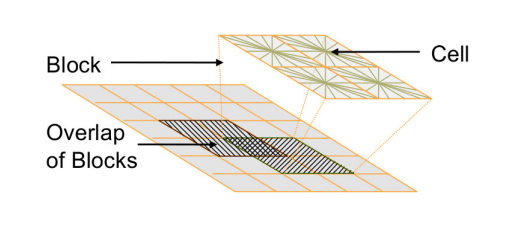
\includegraphics[height=3cm]{blocoverlap.png}}}
\caption{Déplacement d'un bloc.}
\label{fig:blocOverlap}
\end{figure}

\subsection{HOG en cascade}

Pour enrichir notre vecteur caractéristique on peut utiliser HOG en cascade qui combines les HOG de l'image à différentes résolutions. Pour procéder on calcule les HOG sur une successions de sous-régions inclusives et les ajoutons au HOG global, comme décrit dans l'article \cite{qiang_zhu_fast_2006}. De cette manière on ajoute de l'information spatiale à notre descripteur.

\begin{figure}[!htbp]
\center
	\subfloat{{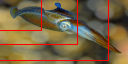
\includegraphics[height=3cm]{Squid_colors_2hogc.png}}}
\caption{HOG en cascade.}
\label{fig:cuttlefish_hog}
\end{figure}




\section{Mesures de similarité}


\subsection{Distance de Bhattacharyya}


\subsection{Cosine similarity}




\section{Filtre à particule}

\begin{algorithm}
	\caption{Filtre à particule}\label{alg:particlefilter}
	\KwData{Une vidéo sous-marine de seiche}
	\KwResult{La liste des positions et bounding box de la cible dans la vidéo}
	\ForEach{Images $t$ de la vidéo}{
		\eIf{Première image}{
			Détection de la seiche dans l'image grâce a YOLOv7\\
			Calcul du descripteur de référence : $F_{ref}^{0}$
		}{
			\ForEach{Particules p}{
				Prédiction de la position et de la bounding box de $p$ dans $t$ en fonction de ses états précédents.\\
				Calcul du descripteur du patch correspondant à $p$ : $F_{p}^{t}$\\
				Calcul du poids de $p$ dans $t$ :
					$$w_{p}^{t} = D_{B}(F_{p}^{t},F_{ref}^{t-1})$$
			}
			Ré-échantillonnage des particules pondérées par leurs poids\\
			Estimation de la position et bounding box de la seiche dans $t$ :
				$$X^{t}=\frac{1}{NB_{particule}}*\sum_{p=0}^{NB_{particule}} x_{p}^{t}*w_{p}^{t}$$
		}
		Mise à jour du descripteur de référence : $F_{ref}^{t}$
	}
\end{algorithm}


\clearpage